\subsection{Dataset and split accounting}
The classification dataset contains 7,112 images. Each class has 1,016
images, with 762 assigned to training and 254 to testing. Within the
training portion, each class contributes 610 fitting samples and 152
validation samples: 4,270 fitting and 1,064 validation samples in total.
The final models are refitted on all 5,334 training images.
No augmentation is applied. Images are converted to grayscale and scaled
to $[0,1]$ for CNN input. The padding alternative centers the image on a
square canvas before nearest-neighbor resizing to $32\times32$.
The original training images are already square, so this padding operation
does not change their geometry; equal validation scores do not establish
that padding has no effect for differently shaped inputs.

\subsection{Recorded software versions}
\noindent platform: macOS-26.5.2-arm64-arm-64bit-Mach-O\\
\noindent python: 3.13.13\\
\noindent torch: 2.14.1\\
\noindent numpy: 2.5.4\\
\subsection{Final CNN training loss}
The curves show training loss only. They do not measure held-out
generalization and are not used to select an epoch using the test data.
\begin{center}
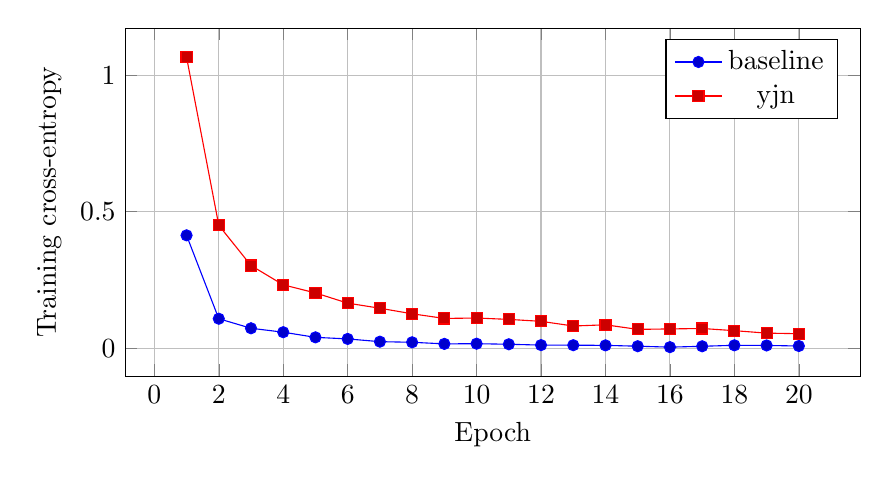
\begin{tikzpicture}
\begin{axis}[width=0.9\linewidth,height=6cm,xlabel={Epoch},ylabel={Training cross-entropy},legend pos=north east,grid=major]
\addplot coordinates {(1,0.4134377773654206) (2,0.10789780974119935) (3,0.07290904862959152) (4,0.05852962733009976) (5,0.03968147791689524) (6,0.033876643598011236) (7,0.023827861122197546) (8,0.021591386175889033) (9,0.01572166312557345) (10,0.016382147748010438) (11,0.014342524904582177) (12,0.011241045239909268) (13,0.010880603854279) (14,0.010308424655303888) (15,0.007189528027239229) (16,0.003782564226846463) (17,0.0069196346105534) (18,0.010523791389057572) (19,0.010016662098712796) (20,0.007931614973573859)};\addlegendentry{baseline}
\addplot coordinates {(1,1.0661209208222422) (2,0.45020170456736464) (3,0.3027684557491534) (4,0.23200079501178053) (5,0.20242419262302472) (6,0.1649499804977178) (7,0.1463364612661724) (8,0.1259487560141118) (9,0.10896114230066549) (10,0.11048587078084023) (11,0.10542576417556004) (12,0.09835842933141206) (13,0.08121352804106051) (14,0.08559057103099114) (15,0.06882336834060775) (16,0.07054128022365101) (17,0.07208789826238428) (18,0.06412577267315757) (19,0.05511437273780907) (20,0.05297138483410566)};\addlegendentry{yjn}
\end{axis}\end{tikzpicture}\end{center}
\subsection{Chip prediction audit}
The table below compares actual predictions with the known reference text.
Reference labels come from the assignment and were not inferred from filenames.
Binary crops are inverted before classification to match the dark-glyph,
white-background polarity of the training images. The uncorrected predictions
are retained in the JSON for traceability. No training or parameter selection
uses these ten crops.
\begin{center}\begin{tabular}{rllll}\toprule
Position & Reference & Baseline & YJN & HOG-SVM \\ \midrule
1 & H & H & 8 & A \\
2 & D & D & 8 & A \\
3 & 4 & 4 & 4 & A \\
4 & 4 & A & 8 & A \\
5 & 7 & 7 & 8 & A \\
6 & 8 & 8 & 8 & A \\
7 & 0 & 0 & 8 & A \\
8 & A & A & A & A \\
9 & 0 & 0 & 8 & A \\
10 & 0 & 0 & 8 & A \\
\bottomrule\end{tabular}\end{center}
baseline: 9/10 position matches; exact-line match: false. yjn: 3/10 position matches; exact-line match: false. hog-svm: 1/10 position matches; exact-line match: false. 

\subsection{Evidence boundaries requiring group review}
The dataset test scores and chip predictions are separate evaluation surfaces.
The tables record high dataset accuracy together with errors on the chip line.
They do not determine the cause of those errors. The group must inspect
segmentation quality, appearance differences and preprocessing choices before
attributing a failure to a particular stage. Only one image and one split seed
are evaluated. The recorded image-level split does not establish independence
across fonts or source images. The earlier smoke run inspected the same test
partition, and the present evaluation must not be described as a new blind test.

\subsection{Timing scope}
CNN training measurements include optimization but exclude loading and
preparing the input tensor. SVM fitting measurements exclude HOG extraction.
Therefore the listed training times are fitting costs, not end-to-end processing
costs. Initial chip timing fields were removed after polarity correction because
they referred to the uncorrected inference run. No corrected latency benchmark
is claimed.
